\section{Proposed method}

\begin{frame}\frametitle{提案手法の概要}
    \begin{columns}
        \begin{column}{0.5\textwidth} % 左:60%
            \begin{block}{要点}
            \begin{itemize}
                \item 映像中全フレームを扱うのは困難なので,compressive sensing
                \item 結果は各ピクセルの改ざんか否か二値映像として構築
            \end{itemize}
            \end{block}
        \end{column}
        \begin{column}{0.5\textwidth} % 右:40%
            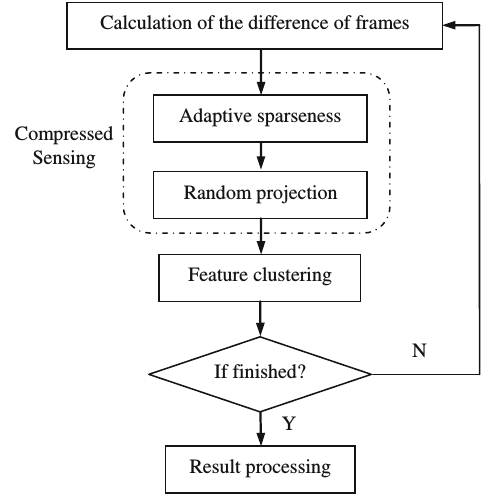
\includegraphics[scale=0.4]{figure/flow.png}
        \end{column}
    \end{columns}
\end{frame}


\begin{frame}{入力データ形式}
\begin{block}{データの変換}
\begin{itemize}
 \item $I$ : 現在のフレーム
 \item $\Delta I$ : $I$ と背景フレームとの差分
 \item $I'$ : K-SVDの入力,下記の変換をかけた $\Delta I$
\end{itemize}
\end{block}
$h_a * h_a$ サイズのブロック列化
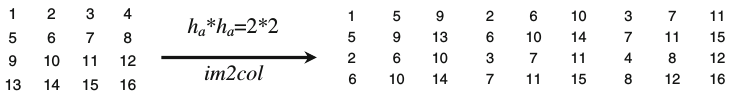
\includegraphics[scale=0.5]{figure/im2col.png}
\end{frame}


\begin{frame}{Adaptive sparseness}
\begin{enumerate}
    \item 辞書 $D$ の DCT 行列による初期化
    \item OMP により $D$ を反復最適化
\end{enumerate}
\end{frame}



\begin{frame}{Random projection}
 
\end{frame}


\begin{frame}{Main working steps}
\begin{enumerate}
    \item $I'$ : 現時刻における差分フレームのブロック表現
    \item $I_{sparse}$ : K-SVD による $I'$ の疎表現
    \item $I_{feature}$ : Gaussian Matrix による射影 $\Theta I_{sparse}$
    \item $\Lambda$ : K-Means による$I_{feature}$ の二値化
\end{enumerate}
\end{frame}
